\documentclass[caret-main.tex]{subfiles}
\begin{document}

\section{Model Metrics}


\subsection{Simple Coin Toss Experiment}

Consider a simple (Fair) Coin Toss experiment. If you were to make a guess as to what the next result is  at each successive throw, you should expect to be right 50\% of the time, after a sufficient number of trials have taken place.
%-----------------------------------------------------------------------------------------------%

\subsection{Kappa Statistic}

% http://www.statistics.com/glossary&term_id=635
Computation of the Kappa Statistic bears a resemblence to the computation of the $\chi^2$ test for independence.
\begin{itemize}
\item The Kappa statistic (or value) is a metric that compares an Observed Accuracy with an Expected Accuracy (random chance).\item The kappa statistic is used not only to evaluate a single classifier, but also to evaluate classifiers amongst themselves. \item In addition, it takes into account random chance (agreement with a random classifier), which generally means it is less misleading than simply using accuracy as a metric (an Observed Accuracy of 80\% is a lot less impressive with an Expected Accuracy of 75\% versus an Expected Accuracy of 50\%). \item Computation of Observed Accuracy and Expected Accuracy is integral to comprehension of the kappa statistic, and is most easily illustrated through use of a confusion matrix.
\item 
The function \texttt{confusionMatrix} can be used to compute various summaries for classification
mode
\end{itemize}
\subsubsection{Computation}
Lets begin with a simple confusion matrix from a simple binary classification of Cats and Dogs:
     Cats Dogs
Cats| 10 | 7  |
Dogs| 5  | 8  |
\begin{itemize}
\item Assume that a model was built using supervised machine learning on labeled data. This doesn't always have to be the case; the kappa statistic is often used as a measure of reliability between two human raters. Regardless, columns correspond to one "rater" while rows correspond to another "rater". 

\item In supervised machine learning, one "rater" reflects ground truth (the actual values of each instance to be classified), obtained from labeled data, and the other "rater" is the machine learning classifier used to perform the classification. Ultimately it doesn't matter which is which to compute the kappa statistic, but for clarity's sake lets say that the columns reflect ground truth and the rows reflect the machine learning classifier classifications.

\item From the confusion matrix we can see there are 30 instances total (10 + 7 + 5 + 8 = 30). According to the first column 15 were labeled as Cats (10 + 5 = 15), and according to the second column 15 were labeled as Dogs (7 + 8 = 15). We can also see that the model classified 17 instances as Cats (10 + 7 = 17) and 13 instances as Dogs (5 + 8 = 13).

\item Observed Accuracy is simply the number of instances that were classified correctly throughout the entire confusion matrix, i.e. the number of instances that were labeled as Cats via ground truth and then classified as Cats by the machine learning classifier, or labeled as Dogs via ground truth and then classified as Dogs by the machine learning model. To calculate Observed Accuracy, we simply add the number of instances that the machine learning classifier agreed with the ground truth label, and divide by the total number of instances. For this confusion matrix, this would be 0.6 ((10 + 8) / 30 = 0.6).

\item Before we get to the equation for the kappa statistic, one more value is needed: the Expected Accuracy. This value is defined as the accuracy that any random classifier would be expected to achieve based on the confusion matrix. The Expected Accuracy is directly related to the number of instances of each class (Cats and Dogs), along with the number of instances that the machine learning classifier agreed with the ground truth label. 
\item To calculate Expected Accuracy for our confusion matrix, first multiply the marginal frequency of Cats for one "rater" by the marginal frequency of Cats for the second "rater", and divide by the total number of instances. \item The marginal frequency for a certain class by a certain "rater" is just the sum of all instances the "rater" indicated were that class. In our case, 15 (10 + 5 = 15) instances were labeled as Cats according to ground truth, and 17 (10 + 7 = 17) instances were classified as Cats by the machine learning classifier. This results in a value of 8.5 (15 * 17 / 30 = 8.5). This is then done for the second class as well (and can be repeated for each additional class if there are more than 2). 15 (10 + 5 = 15) instances were labeled as Dogs according to ground truth, and 13 (10 + 7 = 17) instances were classified as Dogs by the machine learning classifier. This results in a value of 6.5 (15 * 13 / 30 = 6.5). 
\item The final step is to add all these values together, and finally divide again by the total number of instances, resulting in an Expected Accuracy of 0.5 ((8.5 + 6.5) / 30 = 0.5). In our example, the Expected Accuracy turned out to be 50\%, as will always be the case when either "rater" classifies each class with the same frequency in a binary classification (both Cats and Dogs contained 15 instances according to ground truth labels in our confusion matrix).
\item 
The kappa statistic can then be calculated using both the Observed Accuracy (0.60) and the Expected Accuracy (0.50) and the formula:
\end{itemize}
\[Kappa = \frac{observed accuracy - expected accuracy}{1 - expected accuracy}\]

%--------------------------------------------------------------------------------------------------------%

So, in our case, the kappa statistic equals: (0.60 - 0.50)/(1 - 0.50) = 0.20.

As another example, here is a less balanced confusion matrix and the corresponding calculations:

     Cats Dogs
Cats| 22 | 9  |
Dogs| 7  | 13 |
Ground truth: Cats (29), Dogs (22) 
Machine Learning Classifier: Cats (31), Dogs (20) 
Total: (51) 

\begin{itemize}
\item Observed Accuracy: ((22 + 13) / 51) = 0.69 
\item Expected Accuracy: ((29 * 31 / 51) + (22 * 20 / 51)) / 51 = 0.51 
\item Kappa: (0.69 - 0.51) / (1 - 0.51) = 0.37
\end{itemize}
In essence, the kappa statistic is a measure of how closely the instances classified by the machine learning classifier matched the data labeled as ground truth, controlling for the accuracy of a random classifier as measured by the expected accuracy. Not only can this kappa statistic shed light into how the classifier itself performed, the kappa statistic for one model is directly comparable to the kappa statistic for any other model used for the same classification task.

\subsubsection{Interpretation}

There is not a standardized interpretation of the kappa statistic. According to Wikipedia (citing their paper), Landis and Koch considers 0-0.20 as slight, 0.21-0.40 as fair, 0.41-0.60 as moderate, 0.61-0.80 as substantial, and 0.81-1 as almost perfect. Fleiss considers kappas > 0.75 as excellent, 0.40-0.75 as fair to good, and < 0.40 as poor. It is important to note that both scales are somewhat arbitrary. At least two further considerations should be taken into account when interpreting the kappa statistic. First, the kappa statistic should always be compared with an accompanied confusion matrix if possible to obtain the most accurate interpretation. Consider the following confusion matrix:

     Cats Dogs
Cats| 60 | 125 |
Dogs| 5  | 5000|
\newpage
%-------------------------------------------------------------------------------------------------------------------%
The kappa statistic is 0.47, well above the threshold for moderate according to Landis and Koch and fair-good for Fleiss. However, notice the hit rate for classifying Cats. Less than a third of all Cats were actually classified as Cats; the rest were all classified as Dogs. If we care more about classifying Cats correctly (say, we are allergic to Cats but not to Dogs, and all we care about is not succumbing to allergies as opposed to maximizing the number of animals we take in), then a classifier with a lower kappa but better rate of classifying Cats might be more ideal.

Second, acceptable kappa statistic values vary on the context. For instance, in many inter-rater reliability studies with easily observable behaviors, kappa statistic values below 0.70 might be considered low. However, in studies using machine learning to explore unobservable phenomena like cognitive states such as day dreaming, kappa statistic values above 0.40 might be considered exceptional.

So, in answer to your question about a 0.40 kappa, it depends. If nothing else, it means that the classifier achieved a rate of classification 2/5 of the way between whatever the expected accuracy was and 100\% accuracy. If expected accuracy was 80\%, that means that the classifier performed 40\% (because kappa is 0.4) of 20\% (because this is the distance between 80\% and 100\%) above 80\% (because this is a kappa of 0, or random chance), or 88\%. So, in that case, each increase in kappa of 0.10 indicates a 2\% increase in classification accuracy. If accuracy was instead 50\%, a kappa of 0.4 would mean that the classifier performed with an accuracy that is 40\% (kappa of 0.4) of 50\% (distance between 50\% and 100\%) greater than 50\% (because this is a kappa of 0, or random chance), or 70\%. Again, in this case that means that an increase in kappa of 0.1 indicates a 5\% increase in classification accuracy.

Classifiers built and evaluated on data sets of different class distributions can be compared more reliably through the kappa statistic (as opposed to merely using accuracy) because of this scaling in relation to expected accuracy. It gives a better indicator of how the classifier performed across all instances, because a simple accuracy can be skewed if the class distribution is similarly skewed. As mentioned earlier, an accuracy of 80\% is a lot more impressive with an expected accuracy of 50\% versus an expected accuracy of 75\%. Expected accuracy as detailed above is susceptible to skewed class distributions, so by controlling for the expected accuracy through the kappa statistic, we allow models of different class distributions to be more easily compared.

That's about all I have. If anyone notices anything left out, anything incorrect, or if anything is still unclear, please let me know so I can improve the answer.

References I found helpful:

Includes a succinct description of kappa: http://standardwisdom.com/softwarejournal/2011/12/confusion-matrix-another-single-value-metric-kappa-statistic/

%Includes a description of calculating expected accuracy: http://epiville.ccnmtl.columbia.edu/popup/how_to_calculate_kappa.html
\newpage
%-------------------------------------------%
\subsection{ROC Curves}

% What are ROC Cuves?

This type of graph is called a Receiver Operating Characteristic curve (or ROC curve.) It is a plot of the true positive rate against the false positive rate for the different possible cutpoints of a diagnostic test.

An ROC curve demonstrates several things:

It shows the tradeoff between sensitivity and specificity (any increase in sensitivity will be accompanied by a decrease in specificity).
The closer the curve follows the left-hand border and then the top border of the ROC space, the more accurate the test.
The closer the curve comes to the 45-degree diagonal of the ROC space, the less accurate the test.
The slope of the tangent line at a cutpoint gives the likelihood ratio (LR) for that value of the test. You can check this out on the graph above. Recall that the LR for T4 < 5 is 52. This corresponds to the far left, steep portion of the curve. The LR for T4 > 9 is 0.2. This corresponds to the far right, nearly horizontal portion of the curve.
The area under the curve is a measure of text accuracy.

\newpage
%--------------------------------------------%
\begin{figure}
\centering
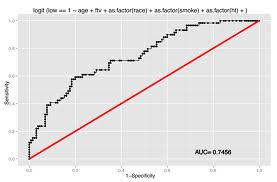
\includegraphics[width=0.4\linewidth]{./ROCcurve}
\caption{}
\label{fig:ROCcurve}
\end{figure}

%--------------------------------------------%
% http://stats.stackexchange.com/questions/24325/lorenz-curve-and-gini-coefficient-for-measuring-classifier-performance

\subsection{The ROC Curve}
The \textbf{\textit{aSAH}} dataset summarizes several clinical and one laboratory variable of 113 patients with an aneurysmal subarachnoid hemorrhage.

\begin{verbatim}
Xavier Robin, Natacha Turck, Alexandre Hainard, et al. (2011) “pROC: an open-source package for R and S+ to analyze and compare ROC curves”. BMC Bioinformatics, 7, 77. DOI: 10.1186/1471-2105-12-77
\end{verbatim}

\begin{verbatim}
> tail(aSAH)
    gos6 outcome gender age wfns s100b  ndka
136    5    Good Female  68    4  0.47 10.33
137    4    Good   Male  53    4  0.17 13.87
138    1    Poor   Male  58    5  0.44 15.89
139    5    Good Female  32    1  0.15 22.43
140    5    Good Female  39    1  0.50  6.79
141    5    Good   Male  34    1  0.48 13.45
\end{verbatim}
%---------------------------------------------%
\begin{itemize}
\item
\item
\end{itemize}
%---------------------------------------------%
\begin{framed}
\begin{verbatim}
library(pROC)
data(aSAH)
# Basic example with 2 roc objects
roc1 <- roc(aSAH$outcome, aSAH$s100b)
\end{verbatim}
\end{framed}

\begin{verbatim}
> roc1

Call:
roc.default(response = aSAH$outcome, predictor = aSAH$s100b)

Data: aSAH$s100b in 72 controls (aSAH$outcome Good) < 41 cases (aSAH$outcome Poor).
Area under the curve: 0.7314

\end{verbatim}

%--------------------------------------------%

% plot(roc1)
% asah-roccurve

\end{document}
